\ac{BOINC} is a system to enable distributed computing and grid computing.
\newline
The organisation who wants other people to provide their computing power to them sets up a \ac{BOINC} server and deploys a project on it. Now people who have the \ac{BOINC} client installed from all around the world can register to the server and participate in projects they find interesting \cite{ries_boinc_2012}.
\newline
The basic idea behind this could also be used for a satellite network.
Every \ac{MCC} who wants to join the network, can set up a \ac{BOINC} server containing the databases with the satellite informations.
Now the \acp{GCC} with the \ac{BOINC} client can connect to the server and poll for jobs. The \ac{MCC} will then see which \acl{GCC} sent the request as the client has to register first. \acl{MCC} checks if the \acl{GCC} meets all the requirements e.g. available bandwidth and resides at the right location for the satellite passing. Hereafter the \ac{MCC} can decide whether to assign the \ac{GCC} or not.
\newline
The \acl{GCC} can then get the orbit data of the respective satellite from the \ac{NASA} \cite{TLE} and enter the received \ac{TLE} in Gpredict (an introduction to Gpredict will be given in section~\ref{sec:gpred_label}) to adjust their antenna rotator. 
\newline
If there is more than one CubeSat passing the \ac{GCC} a scheduler has to be implemented to avoid conflicts and to choose the satellite according to the highest probability of high quality data \cite{preindl_optimization_2010}.
\newline
The received data will be stored at a local database and transmitted to the \ac{BOINC}-server.
After receiving the collected data the server can now crosscheck the results with information provided by other \acp{GCC}.
\begin{figure}[ht!]
\centering
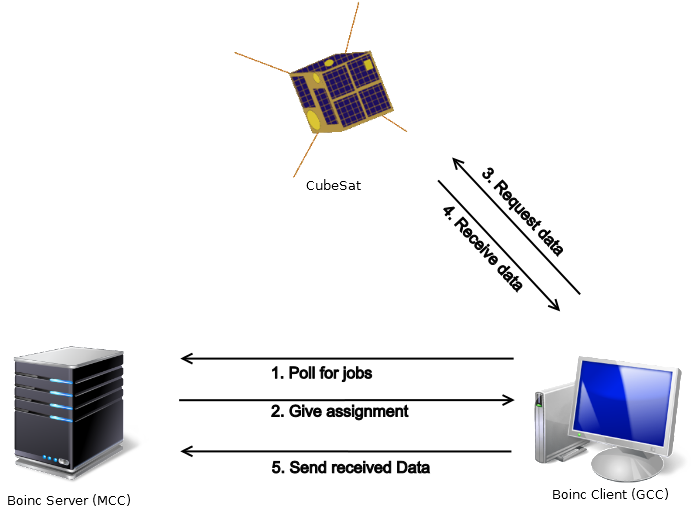
\includegraphics[width=100mm]{PICs/Diagramm1.png}
\caption{\ac{BOINC} illustration \label{BoincIllustration}}
\end{figure}

